\chapter{Food 2}

\begin{itemize}
\tightlist
\item
  \textbf{NP 23,} Over-kept tonics
\item
  \textbf{Pc 39,} Requesting finer staple foods
\item
  \textbf{Pc 47,} Exceeding an invitation
\item
  \textbf{Pc 41,} Handing food to members of other religions
\item
  \textbf{Pd 3,} Protected families
\end{itemize}

\section{NP 23, Over-kept tonics}

\includemap{../../src/includes/mindmaps/np-23-tonics.png}

\begin{multicols}{2}

\textbf{Object:} any of the five tonics.

\textbf{Effort:} one keeps the tonic past the 7th dawnrise after
receiving it.

\textbf{Perception} is not a factor.

If one thinks the 7th dawn haven't passed, but it has, it is still NP.

If one thinks ``I receive \emph{this} salt as food for the morning, and
\emph{this} salt as medicine for later'', it may be a personal practice,
but not part of the rule. It doesn't affect the period of how long the
item may be used by oneself or any other bhikkhu.

\end{multicols}
\par
\enlargethispage{2\baselineskip}

\textbf{Mixing:} The mixture takes on the shortest lifetime of the
ingredients. (Mv. VI.40.3.)

\begin{center}
\begin{tabular}{llllllll}
a. & 1d juice & rec. that morning & + & food & rec. that morning & \(\rightarrow\) & that morning\\
\hline
b. & 7d tonic & rec. that morning & + & food & rec. that morning & \(\rightarrow\) & that morning\\
\hline
c. & lifetime medicine & rec. that morning & + & food & rec. that morning & \(\rightarrow\) & that morning\\
\hline
d. & 7d tonic & rec. sometime & + & juice & rec. that day & \(\rightarrow\) & until dawn\\
\hline
e. & lifetime medicine & rec. sometime & + & juice & rec. that day & \(\rightarrow\) & until dawn\\
\hline
f. & lifetime medicine & rec. sometime & + & 7d tonic & rec. sometime & \(\rightarrow\) & 7 days\\
\end{tabular}
\end{center}

\clearpage

\subsection{7 days}

\emph{Sattāha paramaṃ}, ``up to seven days''. The Vinaya counts days
from dawn to dawn, hence one may use a 7 day tonic \emph{until the 7th
dawn}.

Confusion arises from ``7 days'' meaning either ``for 7 days''
(interval) or ``on the 7th day'' (ordinal).

\vspace*{\baselineskip}

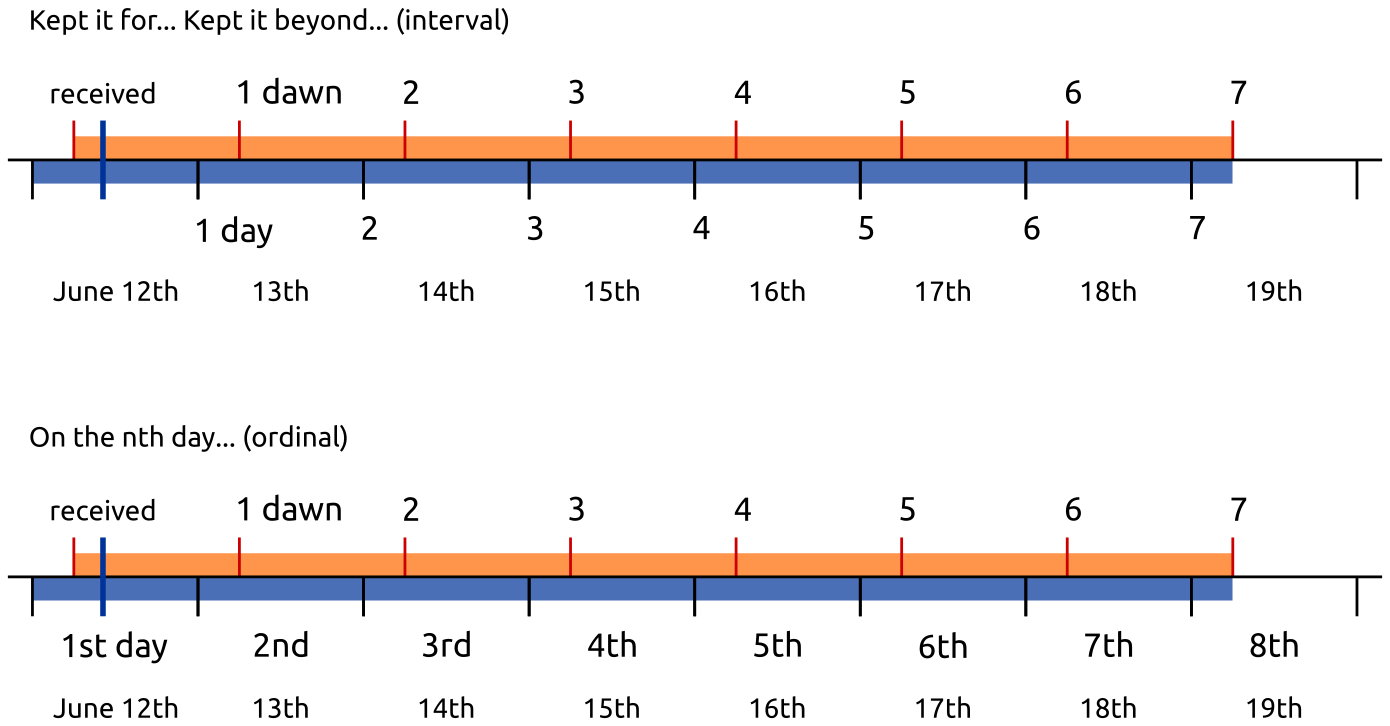
\includegraphics{../../src/includes/figures/7-days.png}

\subsection{Breakfast tray}

After dawn, one receives a tray with bread, jams, honey, butter and
salt. At this point the lifetimes are:

\begin{itemize}
\tightlist
\item
  bread, jams: morning
\item
  honey, butter: 7 days
\item
  salt: lifetime
\end{itemize}

If the knife which one used carries bread morsels or jam into the honey
or the butter, these will be only allowable in the morning.

If one is careful to clean the knife and avoid mixing, one may use them
on the bread and keep the rest until their allowed lifetimes.

The next day, one receives a tray with only bread. One may \textbf{not}
mix the allowables from the previous day with the food received today.

Putting the salt, honey or butter (rec. yesterday) on the bread would be
Pc 38 (eating stored food).

\clearpage

\section{Pc 39, Requesting finer staple foods}

Finer staple foods: ghee, fresh butter, oil, honey, sugar, fish, meat,
milk, curds.

Object, effort, result.

Sk 37 covers non-fine staples: ``Not being ill, I will not eat rice or
bean curry that I have requested for my own sake: a training to be
observed.''

Hence, dukkata for requesting and consuming other staple foods, except
when one is ill.

\subsection{Non-offenses}

\emph{Not ill:} one is able to fare comfortably without these foods.

\begin{multicols}{2}

\begin{itemize}
\tightlist
\item
  being ill
\item
  was requested for the sake of an ill bhikkhu, and is now left over
\item
  from relatives
\item
  from those who gave invitation to ask
\item
  for the sake of another
\item
  from one's own resources
\end{itemize}

\end{multicols}

\section{Pc 47, Exceeding an invitation}

When an invitation is made that one may ask for certain requisites, one
may use it until four months, unless it has been repeated, or is a
permanent invitation.

\subsection{Non-offenses}

\begin{multicols}{2}

\begin{itemize}
\tightlist
\item
  from relatives
\item
  for the sake of another
\item
  from one's own resources
\item
  being ill, if one shows consideration
\end{itemize}

\end{multicols}

``The time period for which we were invited has passed, but we have need
of medicine.''

\section{Pc 41, Handing food to members of other religions}

One places oneself in the position of the followers of other religions.

It is not an offense to prepare food in a tray and placing it so that
they can help themselves.

\section{Pd 3, Protected families}

The purpose is to avoid damaging the faith of those supporters who might
suffer financially if they give too much.

\subsection{Non-offenses}

\begin{multicols}{2}

\begin{itemize}
\tightlist
\item
  being ill
\item
  invited
\item
  juice, tonics, medicines
\item
  the almsfood is supplied by others
\item
  the family members take turns
\item
  eating the leftovers of another bhikkhu
\item
  the family offers outside their residence
\end{itemize}

\end{multicols}

